\chapter{Progettazione}

\noindent La fase di progettazione traduce i requisiti analizzati in una struttura tecnica definita, seguendo un approccio top-down. Inizialmente viene definita l'architettura macroscopica del sistema, per poi scendere nel dettaglio dei singoli componenti e delle loro interazioni dinamiche.

\section{Architettura Logica (Sottosistemi)}

\noindent In conformità con lo sforzo di progettazione ad alto livello richiesto, il sistema è stato suddiviso in \textbf{sottosistemi a compartimenti stagni}. Questa scelta garantisce l'indipendenza funzionale e facilita la manutenzione, permettendo a ogni modulo di evolvere senza impattare direttamente sugli altri.

\noindent L'architettura logica si articola in tre macro-moduli principali:

\begin{itemize}
    \item \textbf{Sottosistema di Presentazione (Frontend)}: Implementa il pattern \textbf{Model-View-Presenter (MVP)} in modalità \textit{Passive View}, assicurando che la logica di visualizzazione sia totalmente disaccoppiata dallo stato dei dati. La \textit{View} notifica gli eventi al \textit{Presenter}, il quale coordina l'aggiornamento del \textit{Model} locale.
    \item \textbf{Sottosistema di Logica di Business (Backend)}: Agisce come coordinatore centrale. Include i moduli \textit{Core} per l'instradamento delle richieste tramite \texttt{Router}, e i \textit{Table Data Gateway} per l'incapsulamento della logica \textit{SQL}. La sicurezza autoritativa è delegata a \textit{Protection Proxies}, mentre la generazione dinamica delle query è affidata al pattern \textit{Strategy}.
    \item \textbf{Sottosistema di Persistenza (Database)}: Modella la base di dati relazionale \texttt{wiki\_db}. L'interazione è mediata dall'astrazione \textit{PDO}. L'accesso a questo modulo è mediato interamente dal backend tramite il pattern \textit{Table Data Gateway}.
\end{itemize}

\noindent La Figura \ref{fig:package_diagram} illustra questa gerarchia attraverso un \textbf{Package Diagram} UML. Le frecce di dipendenza mostrano come il Frontend dipenda dal Backend per il recupero dei dati, e quest'ultimo dipenda dal Database per la persistenza, rispettando il principio del disaccoppiamento.

\begin{figure}[H]
    \centering
    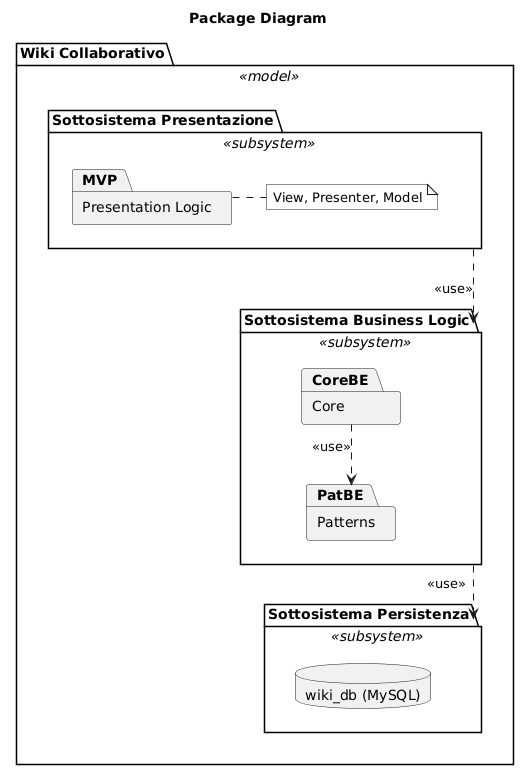
\includegraphics[width=0.7\textwidth]{AltriDiagrammi/PackDiag.png}
    \caption{Package Diagram}
    \label{fig:package_diagram}
\end{figure}

\section{Architettura Fisica (Deployment)}

\noindent L'architettura fisica del sistema è basata sulla tecnologia di containerizzazione \textbf{Docker}, che permette di isolare i sottosistemi in ambienti di esecuzione (nodi) indipendenti e riproducibili. La configurazione è definita tramite il file \texttt{docker-compose.yml}, che orchestra tre container distinti:

\begin{enumerate}
    \item \textbf{Container Frontend}: Utilizza l'immagine \texttt{httpd:alpine}. Espone il servizio sulla porta \textbf{8080} del PC-Host, servendo i file statici (HTML/CSS) e gli script JavaScript al browser dell’utente.
    \item \textbf{Container Backend}: Basato sull'immagine \texttt{php:8.2-apache}. Risponde sulla porta \textbf{8000} e gestisce la logica \texttt{PHP}. Include le estensioni \texttt{pdo\_mysql} necessarie per il dialogo con il database.
    \item \textbf{Container Database}: Utilizza \texttt{mysql:8.0} sulla porta interna \textbf{3306}. La persistenza è garantita da un volume dedicato (\texttt{db\_data}), assicurando che i dati sopravvivano al ciclo di vita del container.
\end{enumerate}

\noindent Tale configurazione soddisfa il requisito \textbf{RNF3 (Indipendenza)}, rendendo il backend e il frontend effettivamente intercambiabili con tecnologie alternative senza compromettere il funzionamento complessivo.

\begin{figure}[H]
    \centering
    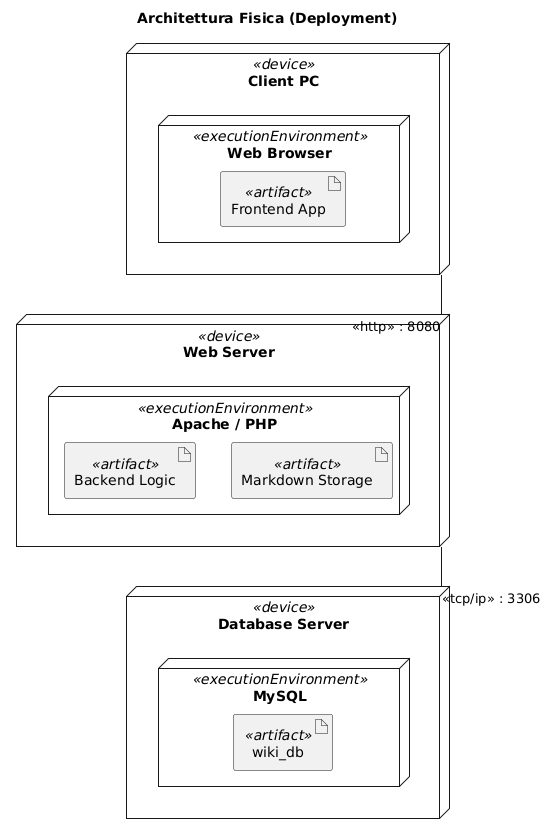
\includegraphics[width=0.6\textwidth]{AltriDiagrammi/deployment.png}
    \caption{Architettura Fisica (Deployment)}
    \label{fig:deployment}
\end{figure}

\section{Processo di Sviluppo e Gestione}

\subsection{Pianificazione delle Attività (Diagramma di GANTT)}

\noindent La pianificazione non segue una rigida successione di fasi, ma è articolata in task basati su obiettivi di progettazione. Ogni task comprende una sotto-fase di modellazione seguita dal refactoring del codice esistente per l'integrazione dei nuovi pattern.

\begin{center}
\begin{ganttchart}[
    expand chart=\textwidth,
    hgrid,
    vgrid,
    x unit=1.2cm,
    y unit title=0.7cm,
    y unit chart=0.8cm,
    title height=1,
    bar/.style={fill=blue!30, draw=blue!60},
    bar height=0.6,
    group/.style={fill=gray!20, draw=black},
    group right shift=0,
    group top shift=0.7,
    group height=.3,
    milestone/.style={fill=red, draw=red},
    milestone height=0.4
]{1}{8} 
    \gantttitle{Pianificazione (W1 - W4)}{8}\\
    \gantttitlelist{1,...,4}{2} \\
    
    \ganttbar{Struttura Iniziale (MVP/TDG)}{1}{1} \\
    \ganttbar{Core Functionality (FE/BE)}{2}{3} \\ 
    \ganttbar{Autenticazione (Strategy)}{4}{4} \\
    \ganttbar{Cronologia (Memento)}{5}{5} \\
    \ganttbar{Sicurezza e Privilegi (Proxy)}{6}{7} \\ 
    \ganttbar{Refactoring e Testing Finale}{8}{8} \\
    \ganttmilestone{Consegna Progetto}{8}
\end{ganttchart}
\captionof{Diagramma di Gantt: Sviluppo Sequenziale del Sistema}
\end{center}

\subsection{Metodologia di Sviluppo}
\noindent Lo sviluppo è stato condotto seguendo una metodologia \textbf{Agile/Scrum} adattata al singolo sviluppatore, caratterizzata da iterazioni brevi e rilasci incrementali di funzionalità (\textit{MVP}). A differenza dei modelli tradizionali, la progettazione architettonica non è stata completata interamente in modo preliminare, ma è evoluta attraverso cicli di \textbf{Refactor Mercilessly} . Questo ha permesso di scoprire la necessità di pattern specifici (come \textit{Memento} o \textit{Proxy}) solo a fronte di reali requisiti emersi durante la codifica, garantendo un design pulito e privo di sovra-progettazione (\textit{YAGNI}). La coerenza del codice è stata mantenuta tramite l'uso di \textbf{Git} per il controllo di versione e \textbf{Docker} per garantire l'uniformità dell'ambiente di esecuzione.

\subsection{Approccio allo Sviluppo}

\noindent Il sistema è stato suddiviso in moduli logici (``tronconi''), i quali rispecchiano la strategia di \textbf{branching} adottata nel repository Git per isolare lo sviluppo delle singole funzionalità prima del merge nel ramo principale. Seguendo un approccio di \textbf{sviluppo incrementale}, ogni passaggio è stato preceduto da una fase di design specifica per garantire che l'implementazione non degradasse la qualità architetturale complessiva.

\begin{itemize}
    \item \textbf{Struttura Iniziale}: Definizione dei pilastri (\textbf{MVP} e \textbf{Table Data Gateway}) per la separazione $FE/BE$ e l'astrazione del DB.
    \item \textbf{Consultazione Appunti}: Stabilite le basi REST API e la gestione del File System.
    \item \textbf{Autenticazione}: Introduzione del pattern \textbf{Strategy} per gestire i criteri di filtraggio utenti e l'hash delle password.
    \item \textbf{Cronologia}: Implementazione del pattern \textbf{Memento} per il salvataggio atomico degli stati storici sul file system.
    \item \textbf{Privilegi e Sicurezza}: Integrazione del pattern \textbf{Protection Proxy} per centralizzare l'autorizzazione senza inquinare la logica dei Gateway.
    \item \textbf{Refactoring Finale}: Scomposizione del \textbf{God Object} \texttt{index.php} in una gerarchia di \texttt{Controller} e \texttt{Router}, ottimizzando la manutenibilità e la "salute" del codice sorgente, abbellimenti al FE, varie fix e aggiunta di qualche funzione extra(come l'anteprima live e il download in pdf).
\end{itemize}

\section{Diagrammi delle Classi}

\noindent I diagrammi delle classi descrivono i tipi di oggetti del sistema e le loro \textbf{relazioni statiche}. Essi formalizzano la struttura del software dettagliando attributi, operazioni e vincoli di ogni componente, comprese le classi che ne definiscono il \textbf{comportamento}.

\subsection{Diagramma delle Classi FE}

\noindent Il diagramma illustra l'architettura del client basata sul pattern \textbf{MVP (Model-View-Presenter)}, finalizzata alla separazione tra logica di presentazione e visualizzazione.

\begin{figure}[H]
    \centering
    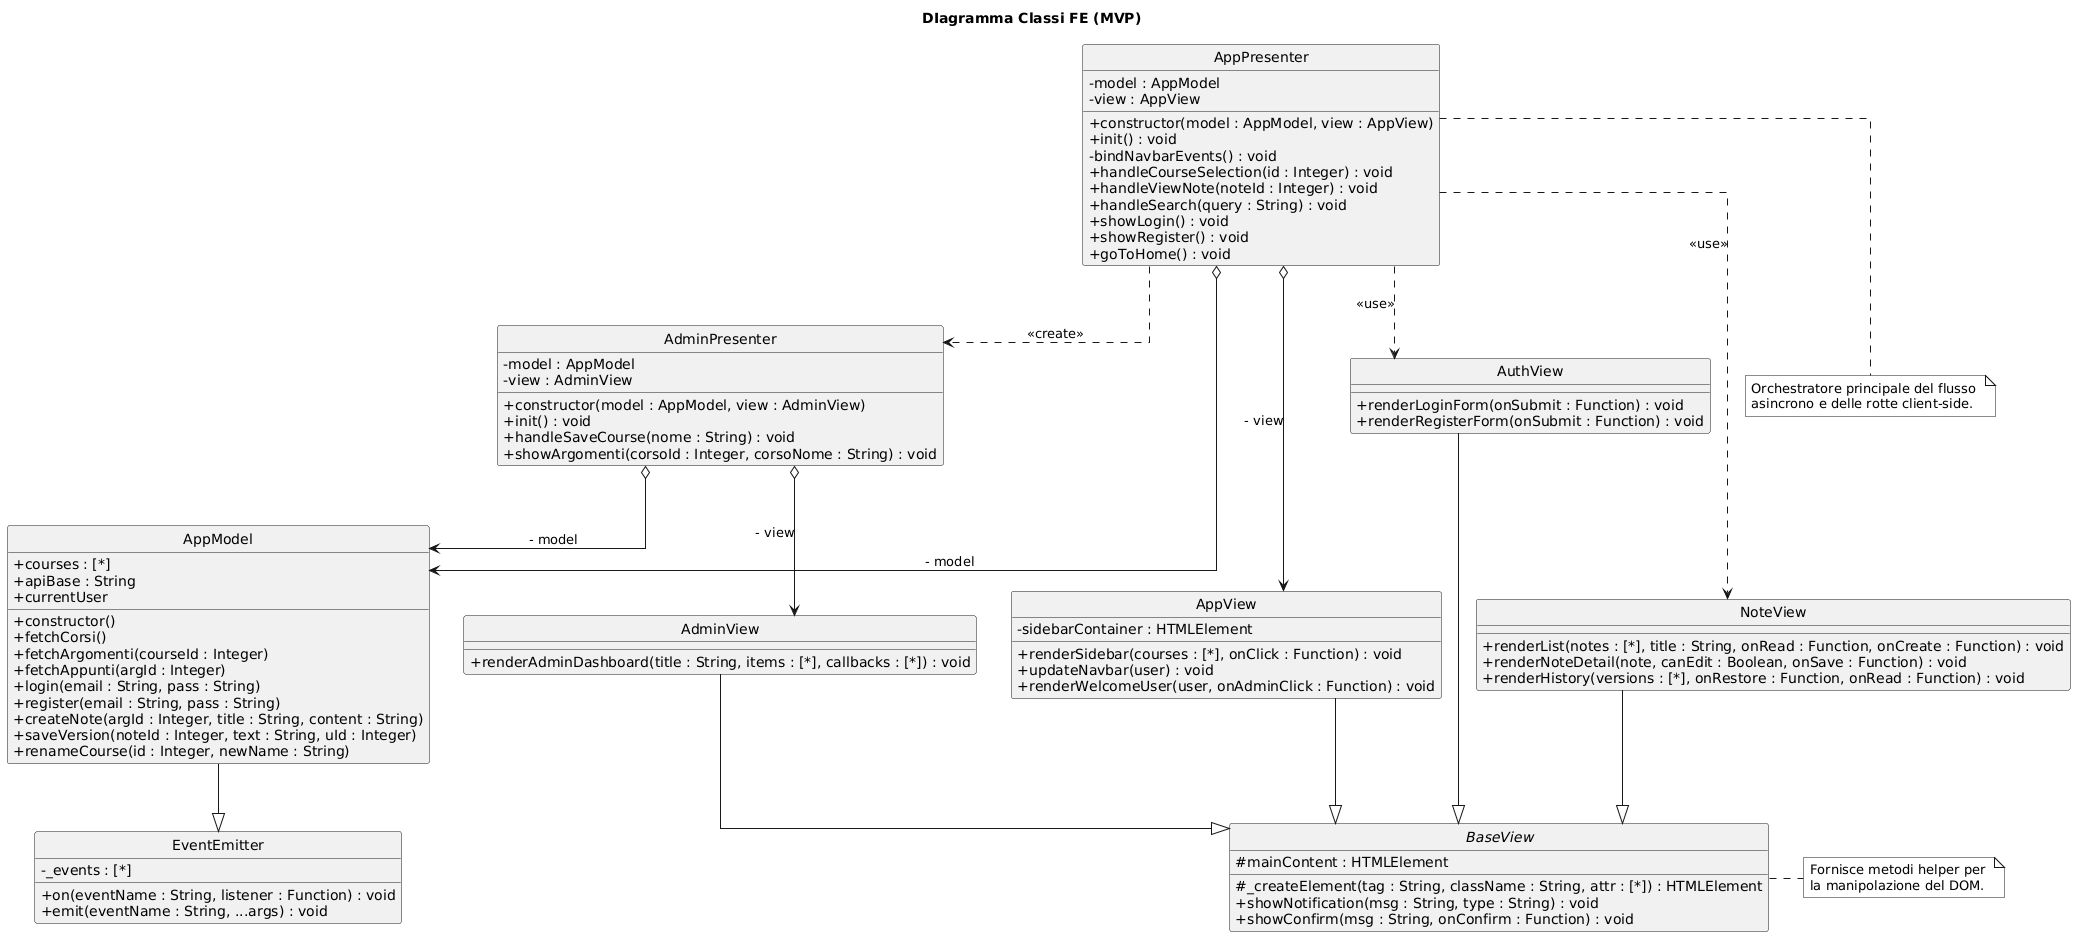
\includegraphics[width=1\textwidth]{DiagrammiClassi/DC_FE.png}
    \caption{FE}
    \label{fig:DC_FE}
\end{figure}

\subsection{Diagramma delle classi BE Sottosistema: Bootstrap \& Orchestration}

Il diagramma delle classi relativo alla fase di \textit{Bootstrap} formalizza l'architettura logica del \textit{Composition Root}, in cui la classe \texttt{Bootstrap} coordina l'intero setup del sistema attraverso relazioni di tipo \guillemotleft create\guillemotright\ verso il \texttt{Router} e la \texttt{DatabaseFactory}. In questo contesto, il meccanismo di instradamento delle richieste è modellato come una \textit{Usage Dependency} (\guillemotleft use\guillemotright) tra il \texttt{Router} e la gerarchia dei controller, riflettendo fedelmente la natura transitoria dell'istanziazione dinamica che avviene all'interno del metodo \texttt{dispatch()}. Al fine di garantire il riuso del codice e la corretta gestione della \textit{Dependency Injection}, è stata introdotta la classe astratta \texttt{BaseController} con funzione di \textit{Layer Supertype}, necessaria a fattorizzare il riferimento al database e ai \textit{Gateway} comuni a tutte le specializzazioni concrete.

\begin{figure}[H]
    \centering
    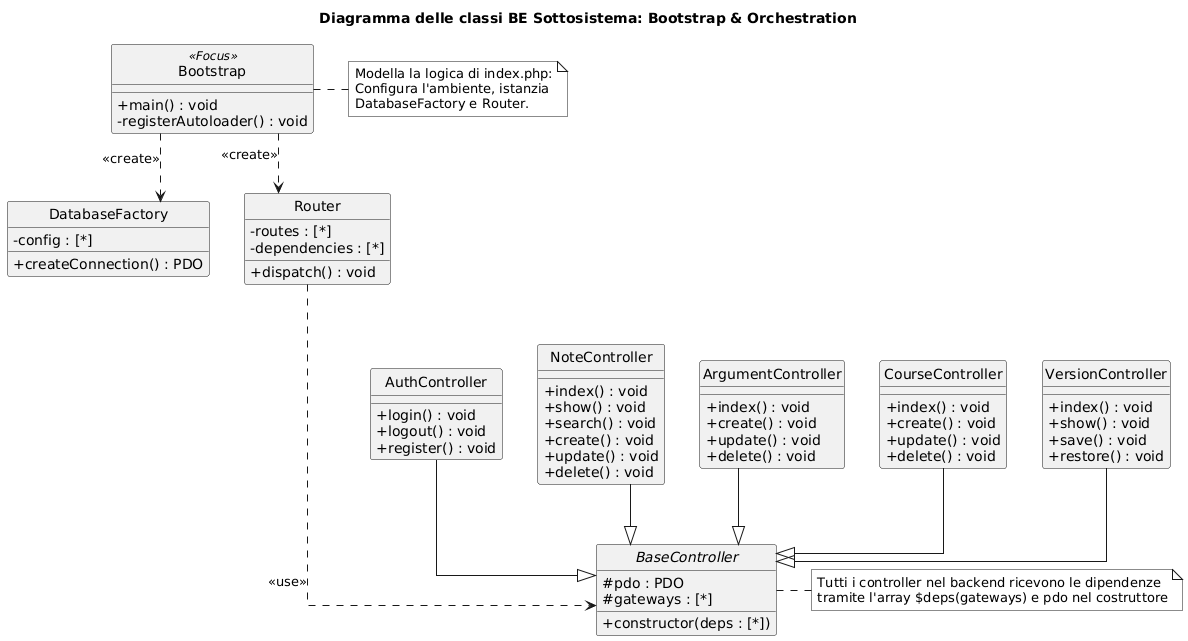
\includegraphics[width=1\textwidth]{DiagrammiClassi/DC_BE_EntryPoint.png}
    \caption{Diagramma delle classi BE Sottosistema: Bootstrap \& Orchestration}
    \label{fig:DC_BE_EntryPoint}
\end{figure}

\subsection{Diagramma delle classi BE Sottosistema: Persistence \& Security}

\noindent Il diagramma del sottosistema di persistenza e sicurezza formalizza l'architettura di accesso allo strato dei dati, strutturata mediante l'integrazione dei pattern \textit{Table Data Gateway} e \textit{Protection Proxy}. Il cuore strutturale è rappresentato dalla gerarchia che discende dalla classe astratta \texttt{AbstractGateway}, la quale centralizza il riferimento protetto all'oggetto \texttt{PDO} e fornisce i metodi necessari per la composizione sicura delle query SQL tramite \textit{Query Object}. In conformità ai requisiti di sicurezza (\textbf{RNF4}), l'accesso operativo ai dati è mediato da una serie di classi \texttt{Proxy} (es. \texttt{NotesGatewayProxy}) che realizzano le interfacce del sottosistema. Tali componenti permettono di intercettare ogni chiamata e verificare i privilegi dell'utente in sessione prima di delegare l'esecuzione effettiva, garantendo così che operazioni sensibili come la creazione o l'eliminazione siano riservate ai soli ruoli autorizzati. Il modulo \texttt{CascadeService} agisce come coordinatore per le procedure di eliminazione complessa, orchestrando l'interazione tra gateway differenti.

\begin{figure}[H]
    \centering
    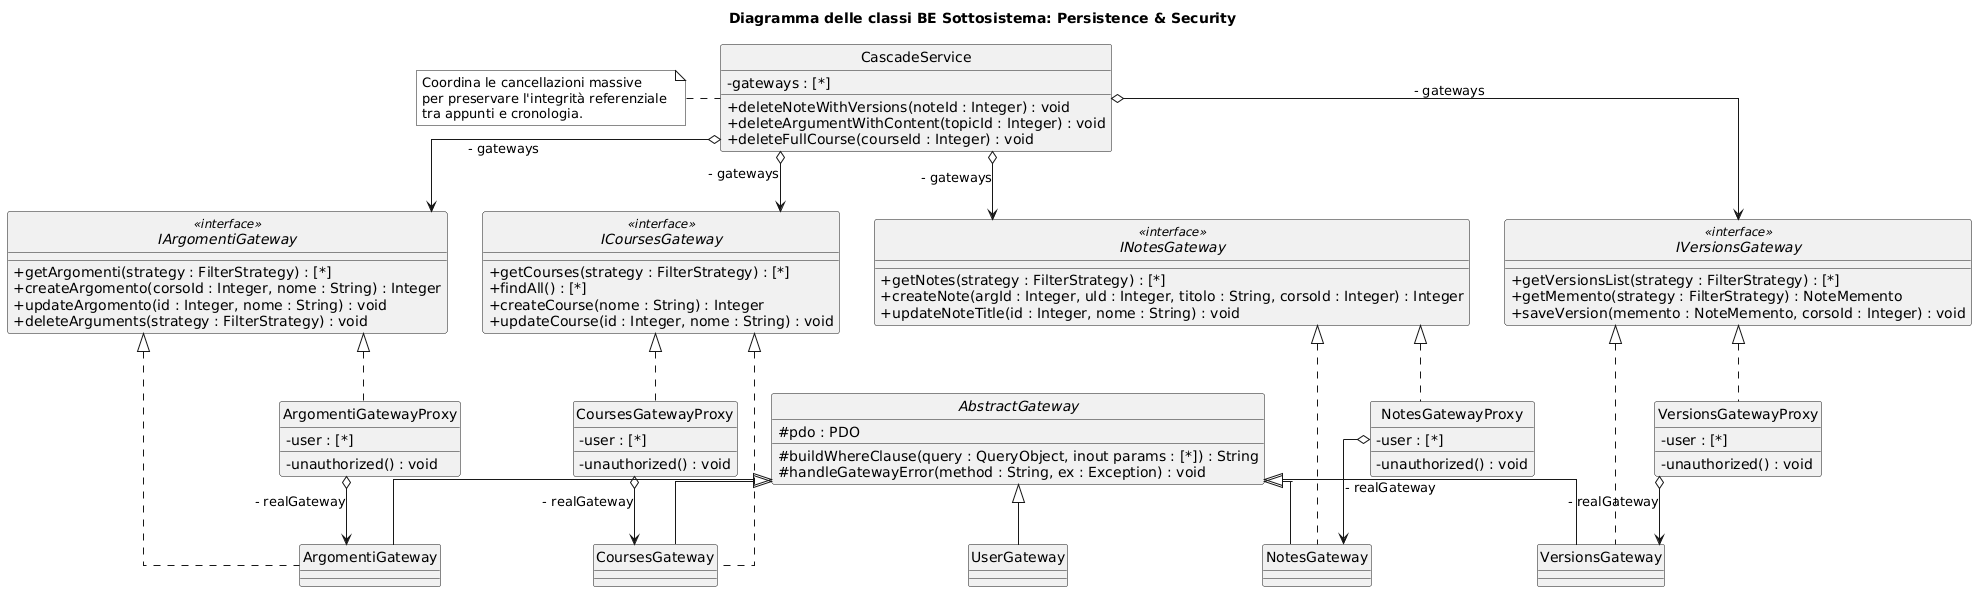
\includegraphics[width=1\textwidth]{DiagrammiClassi/DC_BE_TDG_Proxy.png}
    \caption{Diagramma delle classi BE Sottosistema: Persistence \& Security}
    \label{fig:DC_BE_TDG}
\end{figure}

\subsection{Diagramma delle classi BE Sottosistema: Strategy \& Query Object}

\noindent Il diagramma delle classi relativo al filtraggio delle risorse formalizza l'architettura utilizzata per la generazione dinamica dei criteri di ricerca, basata sull'integrazione dei pattern \textit{Strategy} e \textit{Query Object}. L'interfaccia \texttt{FilterStrategy} funge da astrazione centrale, definendo il contratto operativo \texttt{buildCriteria()} che permette di estendere il sistema con nuovi algoritmi di filtraggio (es. \texttt{SearchFilter} o \texttt{CourseFilter}) senza modificare i client esistenti, rispettando il principio \textit{Open/Closed}. Il disaccoppiamento tra la logica di dominio e la sintassi SQL è garantito dalla classe \texttt{QueryObject}. Tale struttura permette alle strategie concrete di popolare l'oggetto di query con requisiti logici (come l'operatore \texttt{LIKE} o \texttt{IN}), che verranno successivamente interpretati dall'infrastruttura di persistenza per produrre \textit{prepared statements} sicuri, assicurando così l'integrità del sistema contro attacchi di \textit{SQL Injection}.

\begin{figure}[H]
    \centering
    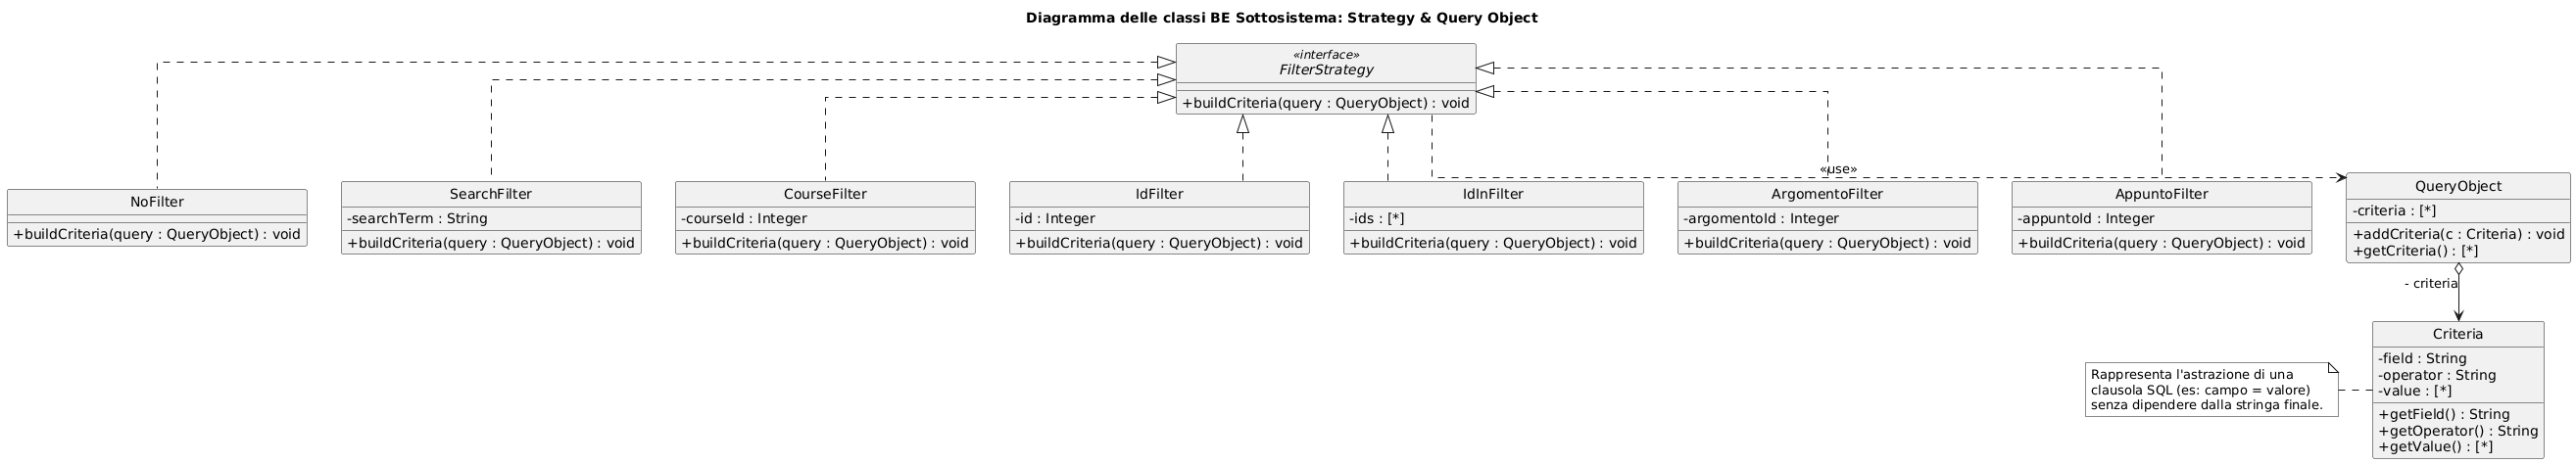
\includegraphics[width=1\textwidth]{DiagrammiClassi/DC_BE_Strategy.png}
    \caption{Diagramma delle classi BE Sottosistema: Strategy \& Query Object}
    \label{fig:DC_BE_Strategy}
\end{figure}

\subsection{Diagramma delle classi BE Sottosistema: Gestione Stato e Cronologia}

Il diagramma delle classi relativo alla persistenza e al ripristino degli appunti formalizza l'applicazione del pattern \textit{Memento}. La classe \texttt{Note} assume il ruolo di \textit{Originator}, detenendo lo stato interno dell'appunto e fornendo i metodi \texttt{saveToMemento()} e \texttt{restoreFromMemento()} per la generazione e il ripristino dei checkpoint. Il legame tra l'originatore e il componente \texttt{NoteMemento} è modellato tramite una \textit{Usage Dependency}, a indicare che la responsabilità dell'istanziazione dello stato spetta esclusivamente alla classe \texttt{Note}. \texttt{NoteMemento} definisce i propri attributi con visibilità privata e li mette a disposizione tramite il metodo \texttt{getState()}, assicurando che lo stato sia accessibile solo per fini di persistenza o ripristino autorizzato. \texttt{VersionsGateway} funge da \textit{Caretaker}, coordinando la custodia e il recupero dei memento dal database.


\begin{figure}[H]
    \centering
    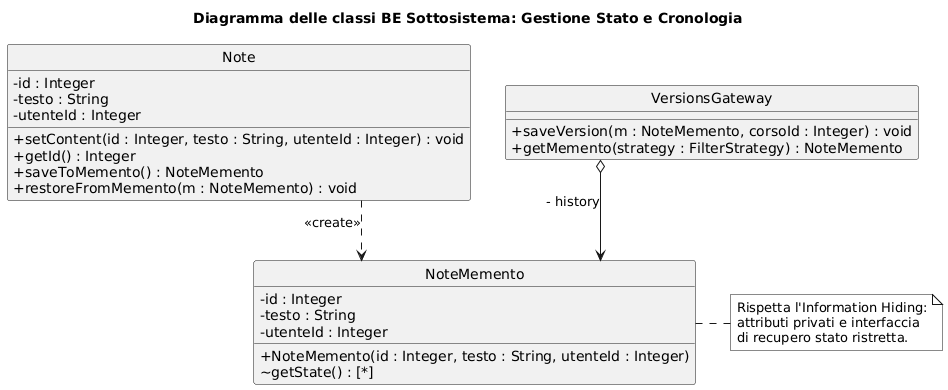
\includegraphics[width=1\textwidth]{DiagrammiClassi/DC_BE_Memento.png}
    \caption{Diagramma delle classi BE Sottosistema: Gestione Stato e Cronologia}
    \label{fig:DC_BE_Memento}
\end{figure}

\section{Diagrammi di Sequenza}

\noindent I seguenti diagrammi mostrano l'interazione temporale tra gli elementi dell'applicativo descrivendo alcuni casi d'uso e mettendo in luce l'uso di alcuni pattern.

\subsection{Diagramma di sequenza: RF6 (Creazione Appunto)}
Il diagramma di sequenza relativo alla creazione di un nuovo appunto formalizza l'integrazione del pattern \textit{Protection Proxy}. Il \texttt{NoteController}, operando come client dell'interfaccia \texttt{INotesGateway}, interagisce in modo trasparente con il \texttt{NotesGatewayProxy} senza conoscere la natura reale dell'oggetto di persistenza. Il cuore del meccanismo di sicurezza risiede nella logica del proxy, il quale intercetta l'invocazione del metodo \texttt{createNote()} e verifica che l'utente in sessione possieda il ruolo di ``studente''. Solo in caso di esito positivo del controllo autoritativo, il proxy delega l'operazione al \texttt{NotesGateway} reale di creazione dell'appunto.

\begin{figure}[H]
    \centering
    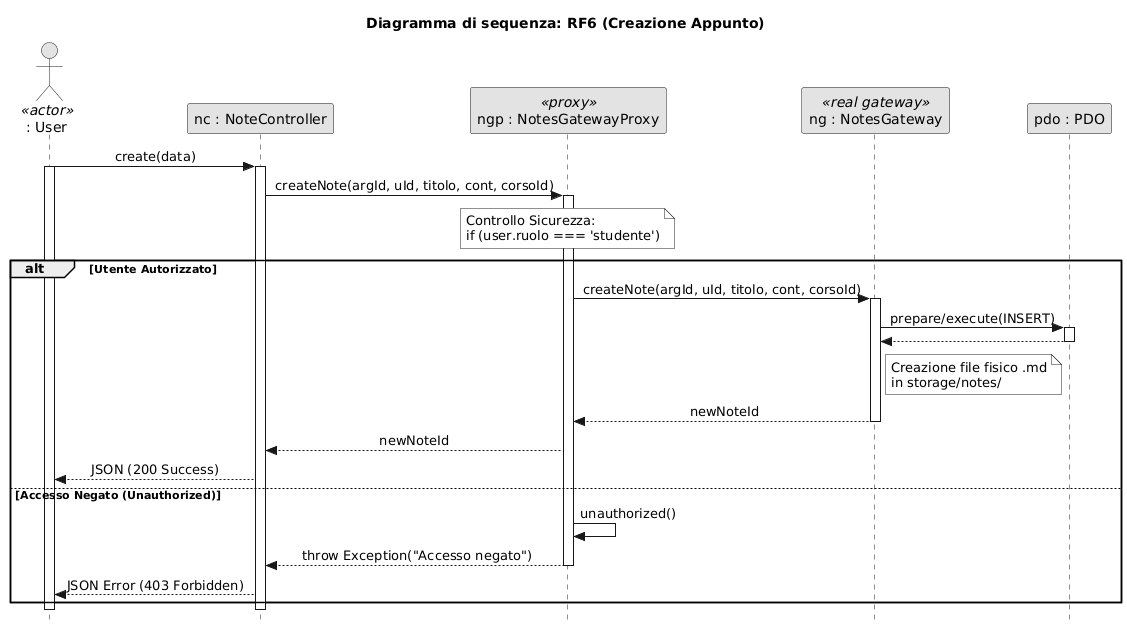
\includegraphics[width=1\textwidth]{DiagrammiSequenza/DS_RF6.png}
    \caption{Diagramma di sequenza: RF6 (Creazione Appunto)}
    \label{fig:DS_RF6}
\end{figure}


\subsection{Diagramma di sequenza: RF8 (parte Salvataggio Nuova Versione)}

Il diagramma di sequenza illustra la procedura di creazione di un checkpoint per un appunto applicando il pattern \textit{Memento}. Il processo è coordinato dal \texttt{VersionController}, il quale, dopo aver aperto una transazione tramite l'astrazione \texttt{PDO}, aggiorna l'oggetto \texttt{Note} (\textit{Originator}) e ne richiede la cattura dello stato tramite il metodo \texttt{saveToMemento()}. Quest'ultimo istanza un oggetto \texttt{NoteMemento} che incapsula le informazioni correnti in modo immutabile. Il \texttt{VersionsGateway} agisce come \textit{Caretaker}, ricevendo il memento e accedendo alla sua interfaccia ``stretta'' tramite il metodo \texttt{getState()} per persistere i dati sul database.

\begin{figure}[H]
    \centering
    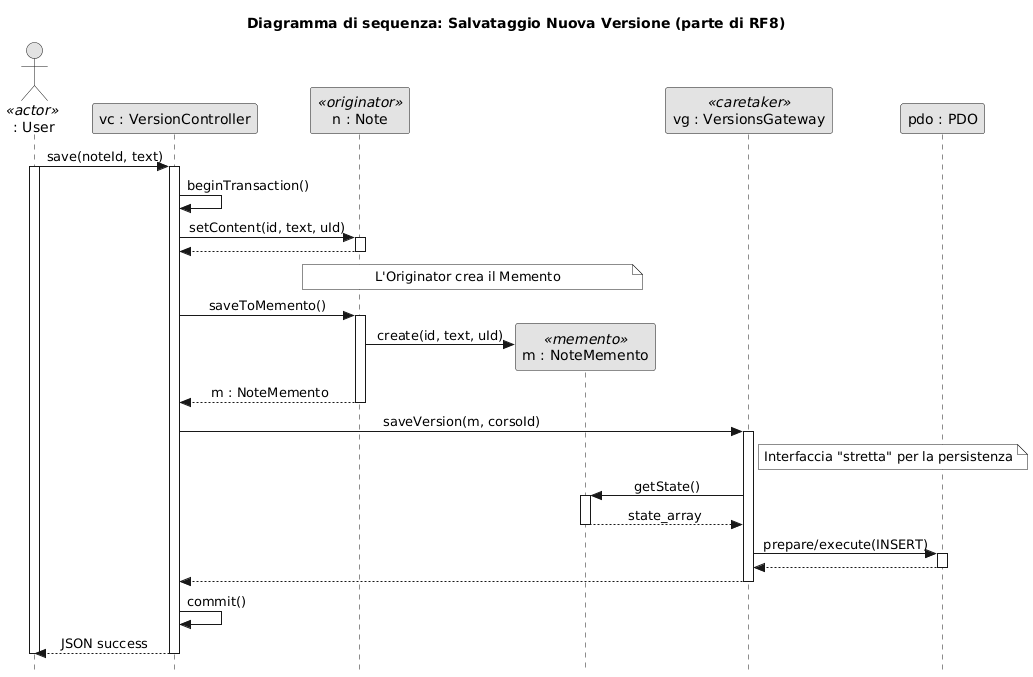
\includegraphics[width=1\textwidth]{DiagrammiSequenza/DS_RF8.png}
    \caption{Diagramma di sequenza: RF8 (parte Salvataggio Nuova Versione)}
    \label{fig:DS_RF8}
\end{figure}

\subsection{Diagramma di sequenza: RF9 (Ricerca Appunti)}

\noindent Il diagramma di sequenza per la ricerca (RF9) illustra l'applicazione del pattern \textbf{Strategy}, garantendo il \textbf{disaccoppiamento} tra logica di controllo e accesso ai dati. Il \texttt{NoteController} istanzia la strategia concreta \texttt{SearchFilter} e la passa al \texttt{NotesGateway} tramite il metodo \texttt{getNotes()}. Il gateway delega alla strategia il popolamento del \textbf{QueryObject} mediante \texttt{buildCriteria()}, applicando l'operatore \texttt{LIKE} sul titolo. Infine, il metodo \texttt{buildWhereClause} trasforma i criteri in un \textbf{prepared statement} SQL sicuro contro la \textbf{SQL Injection}. Questa architettura rispetta il principio \textbf{Open/Closed}, permettendo di aggiungere nuovi filtri senza modificare la struttura del gateway.

\begin{figure}[H]
    \centering
    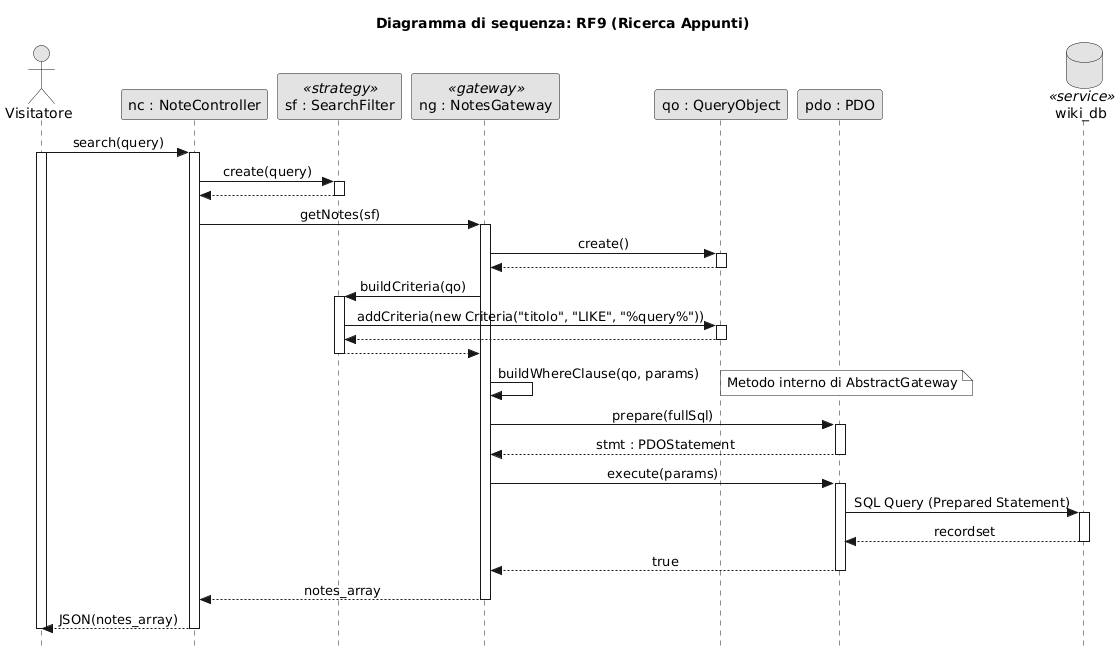
\includegraphics[width=1\textwidth]{DiagrammiSequenza/DS_RF9.png}
    \caption{Diagramma di sequenza: RF9 (Ricerca Appunti)}
    \label{fig:DS_RF9}
\end{figure}

\section{Diagrammi di Attività}

\noindent I diagrammi delle attività descrivono il flusso di controllo e le informazioni dei processi, supportando la modellazione di comportamenti paralleli. Nella progettazione software, questi grafici illustrano algoritmi e operazioni attraverso nodi, archi e partizioni (\textit{swimlanes}) per suddividere le responsabilità tra i componenti.


\subsection{Diagramma delle Attività: Login (RF2)}

\noindent Il diagramma delle attività per il \textbf{login (RF2)} illustra la verifica dell'identità. Il flusso parte dal \texttt{AppPresenter} (validazione sintattica) e passa al \texttt{AppModel}. Nel backend, l'\texttt{AuthController} coordina lo \texttt{UserGateway}, che applica la \textbf{Strategy} \texttt{EmailFilter} per il recupero dei dati. In linea con i requisiti di \textbf{sicurezza (RNF4)}, il sistema confronta l'\textbf{hash sha256} della password fornita con quello memorizzato. Eventuali errori sono gestiti da nodi di decisione che restituiscono uno stato \textbf{HTTP 401 (Unauthorized)}, mentre il successo determina l'avvio della sessione e il reindirizzamento dell'utente.


\begin{figure}[H]
    \centering
    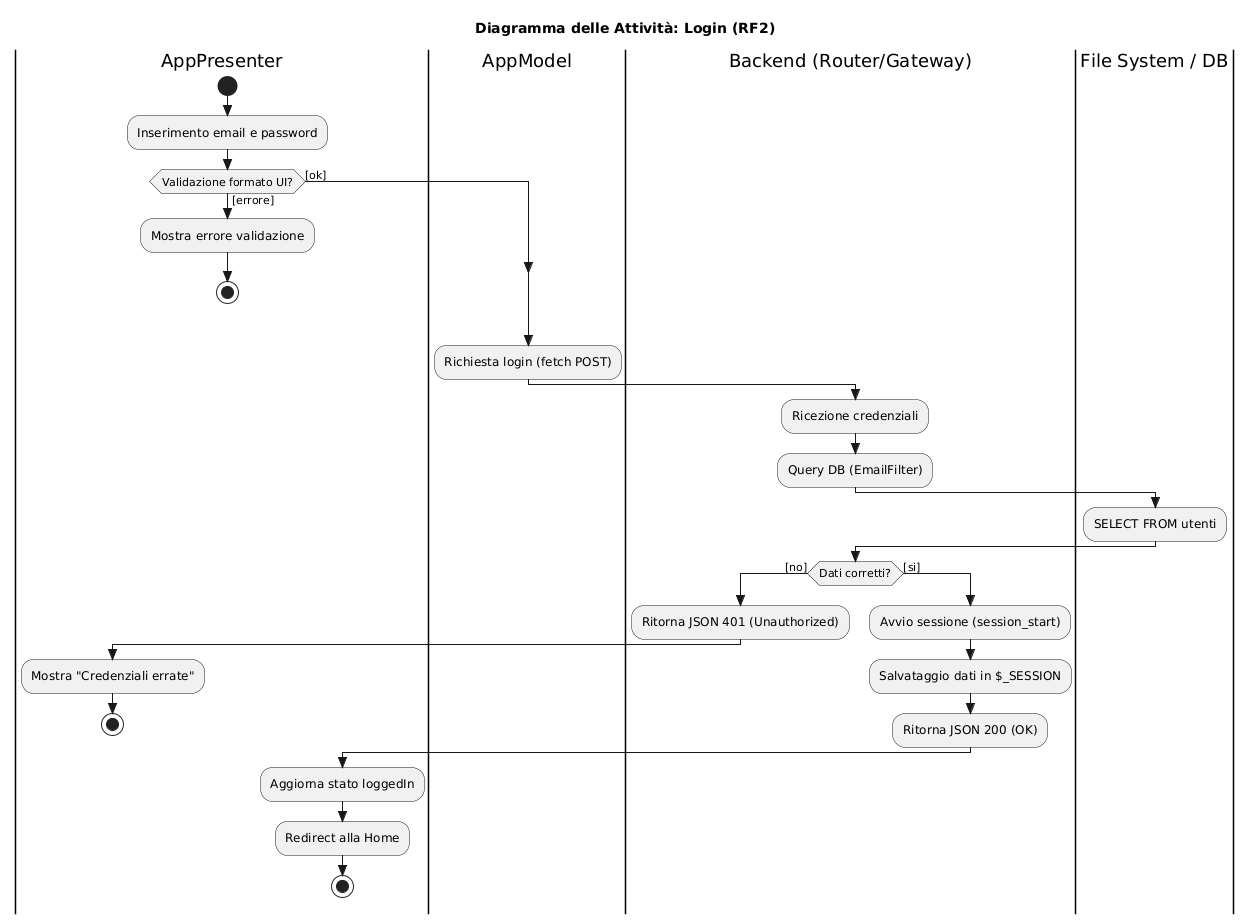
\includegraphics[width=1\textwidth]{DiagrammiAttivita/DA_RF2.png}
    \caption{Diagramma delle Attività: Login (RF2)}
    \label{fig:DA_RF2}
\end{figure}

\subsection{Diagramma delle Attività: Visualizza Appunto (RF5)}

\noindent Il seguente diagramma delle attività illustra il flusso di recupero di un appunto, caratterizzato dalla scomposizione della risorsa tra database relazionale e \textit{file system}. Il processo è innescato dal \texttt{AppPresenter} e mediato dal \texttt{AppModel} tramite una richiesta asincrona allo strato di \textit{backend}. Il \texttt{NotesGateway} esegue una query SQL per estrarre i metadati e il percorso relativo del file; successivamente, una struttura di controllo verifica l'esistenza fisica del documento Markdown nel \textit{file system}. Il punto critico del processo risiede nell'``Integrazione Dati'', fase in cui il gateway aggrega il record del database con il contenuto testuale letto dal disco prima di veicolare la risposta JSON completa verso il \textit{frontend}, garantendo la tracciabilità del requisito RF5 e la gestione degli errori in caso di file mancante.

\begin{figure}[H]
    \centering
    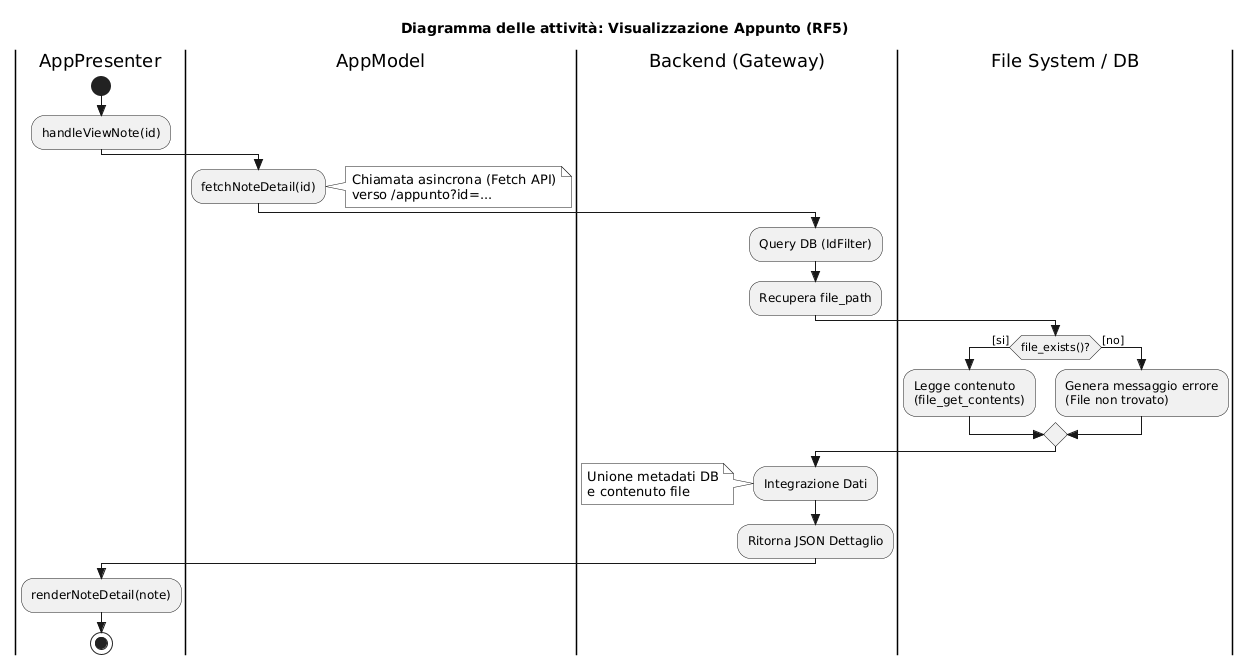
\includegraphics[width=1\textwidth]{DiagrammiAttivita/DA_RF5.png}
    \caption{Diagramma delle Attività: Visualizza Appunto (RF5)}
    \label{fig:DA_RF5}
\end{figure}


\section{Progettazione dei Dati}

\noindent Il sistema adotta un approccio di persistenza ibrido per ottimizzare la gestione di contenuti testuali variabili. Il database relazionale MySQL è incaricato della gestione della struttura logica. Il contenuto effettivo degli appunti e delle loro versioni non viene salvato nelle tabelle, ma archiviato direttamente nel file system del server. All'interno del database, i campi \texttt{file\_path} fungono da puntatori verso i file Markdown fisici, permettendo di unire la velocità di accesso al disco per file voluminosi con la coerenza dei metadati garantita dallo strato \texttt{SQL}.

\begin{figure}[H]
    \centering
    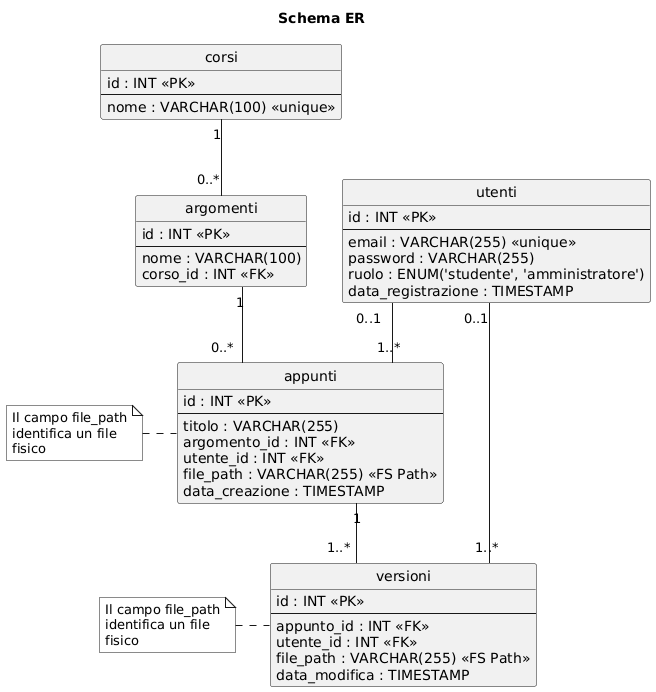
\includegraphics[width=0.8\textwidth]{AltriDiagrammi/DER.png}
    \caption{Schema Entity-Relationship}
    \label{fig:DER}
\end{figure}

\subsection{Organizzazione del File System}

\noindent I file sono organizzati in una struttura a directory che riflette la gerarchia logica del catalogo, facilitando la manutenzione e scalabilità del sistema. La radice del repository è la cartella \texttt{notes} (sotto \texttt{backend/storage/}), strutturata come segue:

\begin{center}
    \begin{minipage}{0.85\textwidth}
        \dirtree{%
        .1 notes/.
        .2 [ID\_Corso]/.
        .3 [ID\_Appunto].md \DTcomment{Versione attuale}.
        .3 versions/.
        .4 [ID\_Appunto]/.
        .5 v1.md \DTcomment{Versioni numerate progressivamente}.
        .5 v2.md.
        }
    \end{minipage}
\end{center}

\noindent L'utilizzo degli ID numerici come nomi di directory e file offre molteplici vantaggi tecnici:
\begin{enumerate}
    \item \textbf{Disaccoppiamento}: Il File System è indipendente dai titoli dei corsi o degli appunti, che possono essere rinominati nel database senza richiedere modifiche ai file.
    \item \textbf{Performance}: La segmentazione in sottodirectory previene il degrado delle prestazioni tipico dei file system con un numero eccessivo di file in un'unica cartella (flat directory).
    \item \textbf{Integrità}: La separazione netta tra la cartella dei contenuti "vivi" e la directory \texttt{versions/} riduce il rischio di sovrascritture accidentali durante le operazioni di manutenzione.
\end{enumerate}

\section{Specifica REST API}

\noindent La comunicazione tra il frontend (\textit{JavaScript}) e il backend (\textit{PHP}) del sistema Wiki Collaborativo avviene attraverso un’architettura di tipo \textbf{RESTful} (Representational State Transfer). Questa scelta garantisce un netto disaccoppiamento tra l'interfaccia utente e la logica di business, permettendo ai due componenti di evolvere indipendentemente e rendendo il sistema facilmente manutenibile e scalabile. Di seguito elenco i principi fondamentali del paradigma \textbf{REST}:

\begin{itemize}
    \item \textbf{Risorse e URI}: Ogni entità del dominio, come \textit{corsi}, \textit{argomenti} e \textit{appunti}, è trattata come una risorsa identificata univocamente da un \textbf{URI} (Uniform Resource Identifier) descrittivo e intuitivo, seguendo una struttura gerarchica coerente.
    
    \item \textbf{Protocollo Stateless}: Ogni richiesta inviata dal client al server è autocontenuta e include tutte le informazioni necessarie per l'elaborazione; al server non è richiesto di memorizzare lo stato del contesto dell'utente tra una chiamata e l'altra, favorendo la scalabilità del sistema.
    
    \item \textbf{Interfaccia Uniforme e CRUD}: Le interazioni avvengono tramite l'uso esplicito dei verbi standard \textbf{HTTP}, che mappano direttamente le operazioni \textbf{CRUD} \textit{(Create, Read, Update, Delete)} sulle risorse: \texttt{GET} per il recupero \textit{(Read)}, \texttt{POST} per la creazione \textit{(Create)}, \texttt{PUT} per l'aggiornamento \textit{(Update)} e \texttt{DELETE} per la rimozione \textit{(Delete)}.
    
    \item \textbf{Formato JSON}: Tutte le risposte prodotte dal backend sono strutturate in formato \textbf{JSON} (JavaScript Object Notation), garantendo un interscambio di dati leggero, facile da leggere per gli umani e semplice da interpretare per le macchine.
\end{itemize}

\noindent Questa interfaccia definisce il contratto formale tra client e server, basato sulla netta \textbf{Separation of Concerns}. Tale approccio assicura che il frontend possa essere teoricamente sostituito con tecnologie alternative (come applicazioni mobile o desktop) senza dover modificare la logica di persistenza e di business implementata nel backend.

\subsection{Endpoint}
Di seguito vengono dettagliati i principali endpoint.

\subsubsection{1. Registrazione utente (RF1)}
\begin{itemize}
    \item \textbf{URL:} \texttt{/register}
    \item \textbf{Metodo:} \texttt{POST}    
    \item \textbf{Parametri Query:} 
        \begin{itemize}
            \item \texttt{email} (obbligatorio).
            \item \texttt{password} (obbligatorio).
        \end{itemize}
    \item \textbf{Descrizione:} Riceve le credenziali dal frontend e crea un nuovo utente.
\end{itemize}
Esempio risposta di Successo (JSON):
\begin{verbatim}
{"status":"success","id":4}
\end{verbatim}

\subsubsection{2. Login (RF2)}
\begin{itemize}
    \item \textbf{URL:} \texttt{/login}
    \item \textbf{Metodo:} \texttt{POST}
    \item \textbf{Parametri Query:} 
        \begin{itemize}
            \item \texttt{email} (obbligatorio).
            \item \texttt{password} (obbligatorio).
        \end{itemize}
    \item \textbf{Descrizione:} Verifica la corrispondenza tra email e password hashata per avviare la sessione.
\end{itemize}
Esempio risposta di Successo (JSON):
\begin{verbatim}
{
    "status": "success",
    "user": {
        "id": 3,
        "email": "nico@studenti.unipr.it",
        "ruolo": "studente",
        "data_registrazione": "2026-01-31 18:18:59"
    }
}
\end{verbatim}

\subsubsection{3. Logout (RF2)}
\begin{itemize}
    \item \textbf{URL:} \texttt{/logout}
    \item \textbf{Metodo:} \texttt{POST}
    \item \textbf{Descrizione:} Invalida la sessione lato server e pulisce lo stato lato client.
\end{itemize}

\subsubsection{4. Visualizzazione Corsi (RF3)}
\begin{itemize}
    \item \textbf{URL:} \texttt{/corsi}
    \item \textbf{Metodo:} \texttt{GET}
    \item \textbf{Descrizione:} Restituisce l'array di tutti i corsi presenti nel database.
\end{itemize}
Esempio risposta di Successo (JSON):
\begin{verbatim}
[
  { "id": 1, "nome": "Informatica" },
  { "id": 2, "nome": "Matematica" }
]
\end{verbatim}

\subsubsection{5. Visualizzazione argomenti di un corso (RF4)}
\begin{itemize}
    \item \textbf{URL:} \texttt{/argomenti}
    \item \textbf{Metodo:} \texttt{GET}
    \item \textbf{Parametri Query:} 
        \begin{itemize}
            \item \texttt{corso\_id} (obbligatorio): Identificativo univoco del corso di riferimento. È un parametro obbligatorio affinché la richiesta vada a buon fine.
        \end{itemize}
    \item \textbf{Descrizione:} Permette di recuperare l'elenco di tutti gli argomenti associati a un determinato corso selezionato dall'utente.
\end{itemize}
Esempio risposta di Successo (JSON):
\begin{verbatim}
[
    {
        "id": 4,
        "nome": "Meccanica",
        "corso_id": 3
    },
    {
        "id": 5,
        "nome": "Termodinamica",
        "corso_id": 3
    }
]
\end{verbatim}


\subsubsection{6. Recupero Appunti per Argomento (RF4,RF5)}
\begin{itemize}
    \item \textbf{URL:} \texttt{/appunti}
    \item \textbf{Metodo:} \texttt{GET}
    \item \textbf{Parametri Query:} 
        \begin{itemize}
            \item \texttt{argomento\_id} (obbligatorio): Identificativo univoco dell'argomento scelto.
        \end{itemize}
    \item \textbf{Descrizione:} Questo endpoint permette di ottenere la lista di tutti gli appunti associati a un determinato argomento. Risponde alla necessità dell'utente di navigare all'interno della gerarchia Corso → Argomento per giungere alla risorsa finale.
\end{itemize}
Esempio risposta di Successo (JSON):
\begin{verbatim}
[
    {
        "id": 4,
        "titolo": "Meccanica Classica",
        "argomento_id": 4,
        "utente_id": 1,
        "file_path": "storage\/notes\/3\/meccanica_classica.md",
        "data_creazione": "2026-01-30 14:53:36"
    },
    {
        "id": 5,
        "titolo": "Meccanica Statistica",
        "argomento_id": 4,
        "utente_id": 1,
        "file_path": "storage\/notes\/3\/meccanica_statistica.md",
        "data_creazione": "2026-01-30 14:53:36"
    }
]
\end{verbatim}

\subsubsection{7. Visualizzazione degli appunti (RF5)}
\begin{itemize}
    \item \textbf{URL:} \texttt{/appunto}
    \item \textbf{Metodo:} \texttt{GET}
    \item \textbf{Parametri Query:} 
        \begin{itemize}
            \item \texttt{id} (obbligatorio): Identificativo univoco dell'appunto scelto.
        \end{itemize}
    \item \textbf{Descrizione:} Restituisce i metadati e il contenuto grezzo del file Markdown.
\end{itemize}
Esempio risposta di Successo (JSON):
\begin{verbatim}
{
    "id": 4,
    "titolo": "Meccanica Classica",
    "argomento_id": 4,
    "utente_id": 1,
    "file_path": "storage\/notes\/3\/meccanica_classica.md",
    "data_creazione": "2026-01-30 14:53:36",
    "contenuto": "# Meccanica classica\r\n\r\nLa **meccanica classica**[...]"
}
\end{verbatim}

\subsubsection{8. Ricerca (RF9)}
\begin{itemize}
    \item \textbf{URL:} \texttt{/cerca}
    \item \textbf{Metodo:} \texttt{GET}
    \item \textbf{Parametri Query:} 
        \begin{itemize}
            \item \texttt{q} (obbligatorio): Rappresenta il termine di ricerca inserito dall'utente. Il sistema backend processa la richiesta solo se la lunghezza di \texttt{q} è maggiore o uguale a 2 caratteri; in caso contrario, viene restituita una lista vuota per ottimizzare le prestazioni
        \end{itemize}
    \item \textbf{Descrizione:} Permette di filtrare la collezione globale degli appunti cercando una corrispondenza testuale all'interno dei titoli.
    \item \textbf{Risposta di Successo (JSON):}
\end{itemize}
\begin{verbatim}
[
    {
        "id": 1,
        "titolo": "Introduzione al Corso",
        "argomento_id": 1,
        "utente_id": 1,
        "file_path": "storage\/notes\/1\/introduzione_al_corso.md",
        "data_creazione": "2026-01-30 14:53:36"
    },
    {
        "id": 6,
        "titolo": "Introduzione alla Termodinamica",
        "argomento_id": 5,
        "utente_id": 1,
        "file_path": "storage\/notes\/3\/introduzione_alla_termodinamica.md",
        "data_creazione": "2026-01-30 14:53:36"
    }
]
\end{verbatim}

\subsubsection{9. Creazione appunti (RF6)}
\begin{itemize}
    \item \textbf{URL}: \texttt{/appunto/crea}
    \item \textbf{Metodo}: POST
    \item \textbf{Parametri Query:}
        \begin{itemize}
            \item \texttt{titolo} (obbligatorio)
            \item \texttt{argomento\_id} (obbligatorio)
            \item \texttt{utente\_id} (obbligatorio)
            \item \texttt{contenuto} (obbligatorio)
        \end{itemize}
    \item \textbf{Descrizione:} Permette a uno studente autenticato di creare un nuovo appunto. Il sistema salva i metadati nel database e crea fisicamente il file \texttt{.md} nello storage dedicato.
    \item \textbf{Risposta di Successo (JSON):}
\end{itemize}
\begin{verbatim}
{ "status": "success", "id": 15 }
\end{verbatim}

\subsubsection{10. Modifica appunti (RF7)}
\begin{itemize}
    \item \textbf{URL}: \texttt{/appunto/versione/salva}
    \item \textbf{Metodo}: POST
    \item \textbf{Body JSON:}
        \begin{itemize}
            \item \texttt{id} (obbligatorio): ID dell'appunto da modificare.
            \item \texttt{testo} (obbligatorio): Nuovo contenuto Markdown.
            \item \texttt{utente\_id} (obbligatorio): ID dello studente che effettua la modifica.
        \end{itemize}
    \item \textbf{Descrizione:} Sovrascrive il contenuto dell'appunto attuale e, contestualmente, applica il pattern \textit{Memento} archiviando lo stato precedente come una nuova versione nella cronologia.
    \item \textbf{Risposta di Successo (JSON):}
\end{itemize}
\begin{verbatim}
{ 
    "status": "success", 
    "message": "Cronologia aggiornata e modifiche salvate" 
}
\end{verbatim}

\subsubsection{11. Gestione corsi, argomenti e appunti (RF10)}
\begin{itemize}
    \item \textbf{URL} (Crea): \texttt{/corso/crea} e \texttt{/argomento/crea} (POST) 
    \item \textbf{URL} (Modifica): \texttt{/corso/modfica}, \texttt{/argomento/modfica} e \texttt{/appunto/modfica} (PUT)
    \item \textbf{URL} (Elimina): \texttt{/corso/elimina}, \texttt{/argomento/elimina} e \texttt{/appunto/elimina} (DELETE)
    \item \textbf{Parametri Body (Esempio Creazione):}
        \begin{itemize}
            \item \texttt{nome} (obbligatorio): Nome della nuova risorsa (corso/argomento).
            \item \texttt{id} (obbligatorio per modifiche ed eliminazioni).
        \end{itemize}
    \item \textbf{Descrizione:} Insieme di API protette dal \textit{Protection Proxy} riservate al ruolo \texttt{amministratore}. Le operazioni di eliminazione utilizzano il \texttt{CascadeService} per garantire la pulizia atomica di DB e File System.
    \item \textbf{Risposta di Successo (JSON):}
\end{itemize}
\begin{verbatim}
{ "status": "success" }
\end{verbatim}

\subsubsection{12. Cronologia delle versioni (RF8)}
\begin{itemize}
    \item \textbf{URL (Lista)}: \texttt{/appunto/storia?id=[ID\_APPUNTO]} (GET)
    \item \textbf{URL (Visualizza)}: \texttt{/appunto/versione/visualizza?versione\_id=[ID]} (GET)
    \item \textbf{URL (Ripristina)}: \texttt{/appunto/versione/ripristina} (POST)
    \item \textbf{Parametri Body (Ripristina):}
        \begin{itemize}
            \item \texttt{versione\_id} (obbligatorio): ID della versione memento da promuovere.
            \item \texttt{utente\_id} (obbligatorio): ID dell'utente che richiede il ripristino.
        \end{itemize}
    \item \textbf{Descrizione:} Gestione dello storico tramite pattern \textit{Memento}. Il ripristino recupera lo stato dal database e dal file system, archiviando lo stato corrente prima di sovrascriverlo.
    \item \textbf{Risposta di Successo (JSON - Ripristina):}
\end{itemize}
\begin{verbatim}
{ 
    "status": "success", 
    "message": "Versione ripristinata correttamente"
}
\end{verbatim}